\PassOptionsToPackage{ukrainian,english}{babel}
\documentclass[onecolumn]{el-author}

%\usepackage[...]{...}      This has been commented out as we are not using any additional packages here.  On the whole, they should be unnecessary.
\usepackage{mathtext}
\usepackage[T1,T2A]{fontenc}
\usepackage[english,ukrainian]{babel}
\usepackage{hyperref}
\usepackage{graphicx} %package to manage images
\usepackage[a4paper, total={7in, 9.5in}]{geometry}
\usepackage{makecell}
\graphicspath{ {images/} }
\newcommand{\hH}{\hat{H}}
\newcommand{\D}{^\dagger}
\newcommand{\ua}{\uparrow}
\newcommand{\nc}{\newcommand}
\renewcommand\theadfont{\normalsize\scshape}
\nc{\da}{\downarrow} \nc{\hc}{\hat{c}} \nc{\hS}{\hat{S}}
\nc{\bra}{\langle} \nc{\ket}{\rangle} \nc{\eq}{equation (\ref}
\nc{\h}{\hat} \nc{\hT}{\h{T}}\nc{\be}{\begin{eqnarray}}
\nc{\ee}{\end{eqnarray}}\nc{\rd}{\textrm{d}}\nc{\e}{eqnarray}\nc{\hR}{\hat{R}}\nc{\Tr}{\mathrm{Tr}}
\nc{\tS}{\tilde{S}}\nc{\tr}{\mathrm{tr}}\nc{\8}{\infty}\nc{\lgs}{\bra\ua,\phi|}\nc{\rgs}{|\ua,\phi\ket}
\nc{\hU}{\hat{U}}\nc{\lfs}{\bra\phi|}\nc{\rfs}{|\phi\ket}\nc{\hZ}{\hat{Z}}\nc{\hd}{\hat{d}}\nc{\mD}{\mathcal{D}}
\nc{\bd}{\bar{d}}\nc{\bc}{\bar{c}}\nc{\mc}{\mathcal}\nc{\ea}{eqnarray}\nc{\mG}{\mathcal{G}}\nc{\bce}{\begin{center}}
\nc{\ece}{\end{center}}
\date{20 Грудня 2018}

\begin{document}

\title{Визначення коефіцієнтів пропускання скляних світлофільтрів}

\author{Сергій Поліщук}

\maketitle

\section{Мета роботи}

вивчення властивостей речовин за їх спектрами пропускання.

\section{Прилади і матеріали}

універсальний об'єктивний фотометр типу ФОУ, набір світлофільтрів.

\section{Завдання}

\begin{enumerate}
	\item при домашній підготовці:
	\begin{itemize}
		\item  користуючись рекомендованою літературою, ознайомитись з
типами світлофільтрів та їх характеристиками;
		\item записати у робочій зошит порядок виконання роботи;
-  зарисувати оптичну схему приладу.
	\end{itemize}
	\item при виконанні роботи:
	\begin{itemize}
		\item  у присутності викладача ввімкнути прилад в електричну
мережу;
		\item  побудувати спектри пропускання трьох світлофільтрів і
порівняти їх з паспортними;
		\item  оформити звіт і подати його викладачеві.
	\end{itemize}
\end{enumerate}

\section{Правила техніки безпеки}

\begin{itemize}
	\item  бережіться пошкодження очей;
	\item  розташуйте прилади таким чином, щоб уникнути їх падіння;
	\item  не торкайтесь пальцями світлофільтрів. Пальці залишають
сліди, що ускладнює виконання роботи.
\end{itemize}

\section{Теоретичні відомості та опис установки}

Світловий потік, спрямований на речовину з деякою прозорістю,
частково відбивається від неї, певна частина його поглинається речовиною,
решта проходить крізь неї.

Відбивання, поглинання і пропускання характеризується відповідними
коефіцієнтами, які, згідно з електронною теорією дисперсії, залежать від
частоти падаючого світла. Зокрема, під коефіцієнтом пропускання $r$
розуміють відношення потоку випромінювання $\Phi$, що пройшов через шар
речовини, до потоку $\Phi _{o}$, що падає на вхідну поверхню. Зазвичай коефіцієнт
пропускання визначають як функцію довжини хвилі $\lambda$. Тоді

\begin{equation} \label{eq:1}
r = \frac{\Phi (\lambda)}{\Phi _{o} (\lambda)}
\end{equation}

Об'єктом дослідження у даній роботі є забарвлені скляні пластинки --
абсорбційні світлофільтри. В оптиці, у загальному розумінні,
світлофільтрами вважаються оптичні пристрої, що володіють вибірковим
спектральним пропусканням і які використовують для ослаблення світла у
бажаних інтервалах довжин хвиль. Найчастіше їх застосовують для
монохроматизації випромінювань і у цьому випадку називають зональними
фільтрами. До цього класу належать абсорбційні, інтерференційні та
дисперсійні світлофільтри. У лабораторних умовах переважно користуються
абсорбційними фільтрами, дія яких основана на вибірковому (селективному)
поглинанні світла. Саме цим пояснюється різний колір поглинаючих
сереловищ. Звідси слідує висновок: якщо речовина селективно поглинає, то
вона і селективно пропускає падаюче на неї випромінювання. Тому здатність
овітлофільтра пропускати слід визначати для різних довжин хвиль, і на
основі виконаних вимірювань побудувати графік залежності $r$ від $\lambda$, що і є
одним із завдань даної роботи. Для реалізації цієї мети універсальний
об'єктивний фотометр  ФОУ обладнаний вісьмома  селективними
поглиначами, характеристики яких зведені у таблицю \ref{tab:1}


\begin{table}[ht]
\label{tab:1}
\caption{\label{tab:1} Характеристики селективних поглиначів фотометру~ФОУ}
{\begin{tabular}{|c|c|c|}\hline
\thead{Номер на рукоятці} & 
\thead{Маркування \\ поглинача} & 
\thead{Приблизне значення \\ довжини хвилі, що \\ відповідає \\ максимальному \\ пропусканню \\ поглинача, нм}\\\hline
1 & 1 & 400 \\\hline
2 & 2 & 457 \\\hline
3 & 3 & 495 \\\hline
4 & 4 & 540 \\\hline
5 & 5 & 585 \\\hline
6 & 6 & 640 \\\hline
7 & 7 & 700 \\\hline
8 & 8 & 750 \\\hline
\end{tabular}}{}
\end{table}

Таким чином, для досліджуваного світлофільтра є можливість
пичначити вісім значень г, що відповідають різним довжинам хвиль.

В основу вимірювань на фотометрі ФОУ покладено принцип
порівняння двох світлових потоків шляхом зміни одного з них за допомогою
пимірювальної діафрагми із змінним отвором.
Зовнішній вигляд приладу ілюструє рис.\ref{img:1}.

На вимірювальних барабанах, зв'язаних з діафрагмами, нанесено
відношення (у процентах) площі отвору діафрагми при даному її відкритті до
площі при максимальному розкритті.

Вимірювання коефіцієнта пропускання полягає в тому, що на
фотоелементи, які включені за диференціальною схемою, направляється
почергово спочатку повний світловий потік, а потім потік, пропущений через
досліджуване середовище. Так як світловий потік рівномірного пучка світла,
який проходить крізь діафрагму, пропорційний площі її розкриття, то
відношення площ отворів відповідає відношенню потоків. Оптична схема фотометра ФОУ зображена на рис.\ref{img:2}.

Світловий пучок від джерела 1 (рис.\ref{img:2}) розділяється дзеркалами
(на схемі не показані) на дві частини, спрямовується на конденсор 2,
паралельним пучком потрапляє на дзеркало 3 і потім проходить крізь
досліджуваний зразок, вимірювальну діафрагму 4, об'єктив 5, відбивається
від дзеркала 6, проходить через один із змінних селективних поглиначів 7
і фокусується на матовому склі 8, яке розміщене перед фотоелементом 9.

Дзеркала 3 і 6 призначені для повертання пучків світла з метою
зменшення розмірів фотометра.

Дзеркало 3 повертає пучки променів на кут 45$^{o}$, направляючи їх на
вимірювальні діафрагми 4. Розсувні вимірювальні діафрагми 4, при
повертанні зв'язаних з ними барабанів, змінюють площу отвору і тим самим
змінюють інтенсивність світлових потоків, падаючих відповідно на лівий і
правий фотоелементи.

Дзеркала 6 направляють два пучки крізь один поглинач, при цьому
пучки перетинаються під кутом 46$^{o}$. Вибіркові поглиначі призначені для
виділення спектральних ділянок в області спектру від 400 до 750 нм і
вводяться в оптичну схему в залежності від вимірів на фотометрі.

На барабані 7 (рис.\ref{img:1}) нанесено дві шкали. Одна шкала має чорний
колір, вона називається шкалою пропускання, на ній показані відношення
$\frac{S}{S_{o}}$ 
у процентах, де $S$ площа розкриття діафрагми при вимірюванні, $S_{o}$ --
площа максимального розкриття діафрагми.

Інша шкала -- червона -- відповідає оптичній густині зразка, під якою
розуміють десятковий логарифм величини, оберненої до коефіцієнта
пропускання. Тобто $D = -lg~r$. Якщо, наприклад, $r = 0.10(10\%)$, то $D=1$.

З правого боку оптичної головки знаходиться ручка 11, якою почергово
уводять у хід променів той чи той поглинач. Цифри на шкалі вказують номер
поглинача, Положення кожного поглинача фіксується.

З лівого боку оптичної головки розміщена ручка 10, поворотом якої
можна збільшити чутливість приладу приблизно у 1,10,100,1000 і у 10000
разів. Цифра «1» відповідає мінімальній чутливості, цифра «5» --
максимальній. Плавно змінювати чутливість можна ручкою 2.

\section{Послідовність виконання роботи}

\begin{enumerate}
	\item Ввімкнути в мережу блок живлення. Час його прогрівання не
менше 15 хвилин. Діафрагми вимірювальних барабанів при
цьому повинні бути повністю відкритими.
	\item Ручку чутливості встановити у положення «1» (груба чутливість).
	\item Після закінчення прогрівання закрити діафрагми і встановити
стрілку мікроамперметра в нульове положення.

УВАГА! При вимірюванні коефіцієнтів пропускання категорично
забороняється обертати барабан 8 (рис.\ref{img:1})).
	\item Правий барабан встановити на поділку «100» чорної шкали, а
досліджуваний зразок помістити у правий пучок світла.
Повертанням лівого барабана встановити положення
фотоелектричної рівноваги («0» на мікроамперметрі). Після
цього зразок вийняти і знову встановити фотоєлектричну
рівновагу шляхом повертання правого барабана. Відлік, взятий
по чорній шкалі цього барабана, дасть коефіцієнт пропускання
даного зразка, а по червоній - його оптичну густину.

Слід відмітити, що фотометр являє собою симетричну
оптичну систему і порядок вимірювань може бути змінений у
тому розумінні, що там, де згадується про правий вимірювальний
барабан (чи діафрагму), можна мати на увазі лівий барабан (чи
діафрагму) і навпаки.

Примітка. Під час вимірювання може статись, що при
встановленні правого барабана на поділку «100» лівим барабаном
не вдається досягнути «0» на мікроамперметрі. Це відбувається
через різну чутливість фотоелементів.

У такому разі на поділку «100» слід встановити шкалу
лівого барабана, досліджуваний зразок помістити у ліве плече
фотометра, а правим барабаном виконати встановлення
електричного нуля.
	\item Для одержання спектральної характеристики світлофільтра В
оптичну схему послідовно ввести селективні поглиначі і
виміряти, згідно п. 4, коефіцієнти пропускання з кожним
поглиначем. На міліметровому папері побудувати  графік-
характеристику пропускної здатності світлофільтра, відкладаючи
довжини хвиль на горизонтальній вісі, а значення $r$ - на
вертикальній. Одержаний результат порівняти з паспортним,
проаналізувати можливі розходження.
	\item Побудувати графічну залежність $r = f(\lambda)$ щонайменше для трьох
світлофільтрів.
\end{enumerate}

\newpage

\begin{thebibliography}{}

\bibitem{1}
Кучерук І.М., Горбачук І.Т. Загальний курс фізики: Т.3.: Оптика.
Квантова фізика. - К.: Техніка, 2006. -- 518с., ст. 101 - 102,
203 - 204.

\bibitem{2}
Кучерук І.М, Дущенко В.П. Загальна фізика. Оптика. Каантоції
фізика. - К.: Вища школа, 1991, -- 463с., ст. 58 - 60, 206 - 215,
224 - 227.

\bibitem{3}
Горбачук І.Т. Загальна фізика. Лабораторний практикум. - К.:
Вища школа, 1992.- 512 с., ст. 450 - 453.

\bibitem{4}
Методична розробка до роботи.

\end{thebibliography}

\section{Завдання для самоконтролю}

\begin{enumerate}
	\item Які світлофільтри відносяться до зональних?
	\item Які фільтри називаються інтерференційними, яка їх будова?
	\item Де застосовуються світлофільтри?
	\item Що таке коефіцієнт пропускання?
	\item Що таке оптична густина напівпрозорого тіла?
	\item У чому полягає вимірювання коефіцієнтів пропускання
відносним та абсолютним методами?
	\item Яку роль відіграють селективні поглиначі?
	\item У якому діапазоні довжин хвиль працює фотометр ФОУ?
	\item Які основні блоки фотометрів типу ФОУ?
	\item Поясніть оптичну схему приладу?
\end{enumerate}

\clearpage
\section{Тестові завдання для вхідного контролю}

\begin{enumerate}
	\item  Під світлофільтром розуміють прилад, який пропускає лише фотони,
певною мірою узгодження за:
	\begin{enumerate}
		\item фазою;
		\item амплітудою;
		\item частотою;
		\item орієнтацією у просторі.
	\end{enumerate}
	\item  В основу дії світлофільтра може бути покладене:
	\begin{enumerate}
		\item селективне поглинання речовиною світла;
		\item вибіркове відбивання світла речовиною;
		\item  розсіювання світла речовиною;
		\item інтерференція світла.
	\end{enumerate}
	\item Яке з цих тперджень хибне? Прозорість речовини залежить від її здатності:
	\begin{enumerate}
		\item поглинати світло;
		\item розсійювати світло;
		\item відбивати світло;
		\item поглинати, розсіювати та відбивати світло.
	\end{enumerate}
	\item Прозорість білого паперу близька до:
	\begin{enumerate}
		\item 0
		\item 0.25
		\item 0.78
		\item 1
	\end{enumerate}
	\item Чи тотожні між собою значення прозорості та коефіцієнта
пропускання світла речовиною?
	\begin{enumerate}
		\item тотожні;
		\item прозорість більша коефіцієнта пропускання;
		\item прозорість менша коефіцієнта пропускання;
		\item прозорість може бути як більшою, так і меншою коефіцієнта
пропускання.
	\end{enumerate}
	\item Чи залежить спектральна ширина смуги пропускання від типу світлофільтра?
	\begin{enumerate}
		\item не залежить;
		\item вона вужча в інтерференційних фільтрах;
		\item ширина смуги пропускання найвужча в абсорбційних фільтрах;
		\item найменшу ширину смуги пропускання дають дисперсійні
світлофільтри.
	\end{enumerate}
	\item Сучасні світлофільтри мають ширину смуги пропускання:
	\begin{enumerate}
		\item 10 нм
		\item 1 нм
		\item 0.1 нм
		\item 0.01 нм
	\end{enumerate}
	\item Фотометр ФОУ працює у такому діапазоні довжин хвиль:
	\begin{enumerate}
		\item 380-760 нм;
		\item 420-740 нм;
		\item 400-750 нм; 
		\item 440-730нм.
	\end{enumerate}
	\item На аркуші паперу мифнь написи червоним, зеленим і синім
фломастером. Який вони матимуть вигляд, якщо їх розглядати через
червоний світлофільтр?
	\begin{enumerate}
		\item всі написи здаватимуться чорними;
		\item червоного напису не буде видно, а зелений і синій будуть чорними;
		\item буде видно лише червоний напис;
		\item всі написи здаватимуться червоними.
	\end{enumerate}
\end{enumerate}

\newpage

\section{Тестові завдання для підсумкового контролю}

\begin{enumerate}
	\item Світлофільтри -- оптичні пристрої, дія яких грунтується на
селективному:
	\begin{enumerate}
		\item пропусканні світла;
		\item відбиванні світла;
		\item пропускайнні або відбиванні світла;
		\item відбиванні або розсіюванні світла.
	\end{enumerate}
	\item Досліджувані у даній роботі світлофільтри відносяться до:
	\begin{enumerate}
		\item абсорбційних;
		\item інтерференційних;
		\item дисперсійних;
		\item емісійних.
	\end{enumerate}
	\item До зональних світлофільтрів належать:
	\begin{enumerate}
		\item лише інтерференційні фільтри;
		\item виключно дисперсійні фільтри;
		\item дисперсійні і абсорбційні фільтри;
		\item  абсорбційні, дисперсійні та інтерфенційні фільтри.
	\end{enumerate}
	\item Абсолютно прозорим є середовище, яке:
	\begin{enumerate}
		\item не відбиває світло;
		\item нерозсіює світло;
		\item не поглинає світло;
		\item має показник заломлення, рівний 1.
	\end{enumerate}
	\item  Коефіцієнт поглинання середовища а залежить:
	\begin{enumerate}
		\item лише від хімічної природи середовища;
		\item від частоти падаючого світла та його інтенсивності;
		\item від товщини шару поглинання та інтенсивності падаючого світла;
		\item від хімічного складу середовища та довжини падаючої хвилі.
	\end{enumerate}
	\item Які з нижче перелічених величин належать до основних характеристик
світлофільтрів: 1) хімічна природа середовища, 2) агрегатний стан,
3) спектральна ширина, 4) прозорість, 5) довжина хвилі 1,,,, 6) оптична
густина?
	\begin{enumerate}
		\item перша, третя і шоста;
		\item друга, четверта та п'ята;
		\item третя, четверта, п'ята та шоста;
		\item всі шість.
	\end{enumerate}
	\item Із яких нижче перелічених речовин виготовляють світлофільтри для
видимої області: 1) кварц, 2) скло, 3) желатин, 4) пластмаса, 5) кристали,
6) рідини?
	\begin{enumerate}
		\item кварц, скло, кристали, рідини;
		\item  скло, желатин, рідини, кристали;
		\item скло, желатин, пластмаса, рідини;
		\item рідини, кристали, кварц, желатин.
	\end{enumerate}
	\item Для яких світлофільтрів оптична густина не залежить від довжини хвилі?
	\begin{enumerate}
		\item абсорбційних;
		\item дисперсійних;
		\item інтерференційних;
		\item нейтральних.
	\end{enumerate}
\end{enumerate}

\clearpage

\begin{figure}[h]
\centering{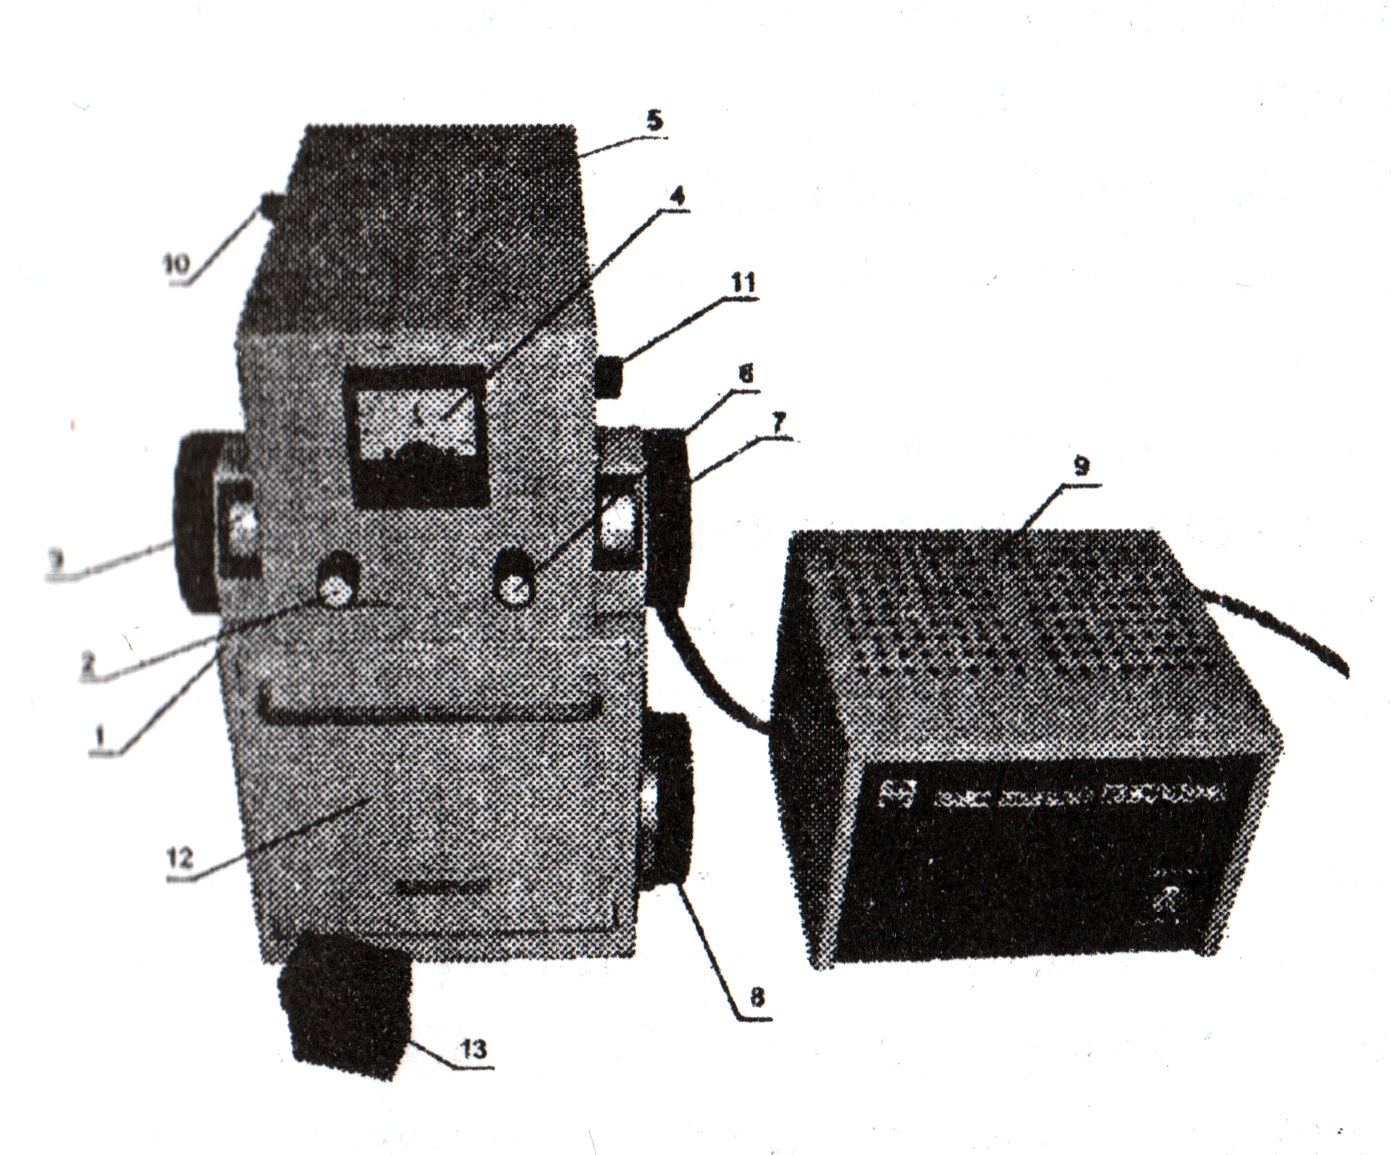
\includegraphics[width=80mm]{img_1}}
\caption{\source{}}
\label{img:1}
\end{figure}

\begin{figure}[h]
\centering{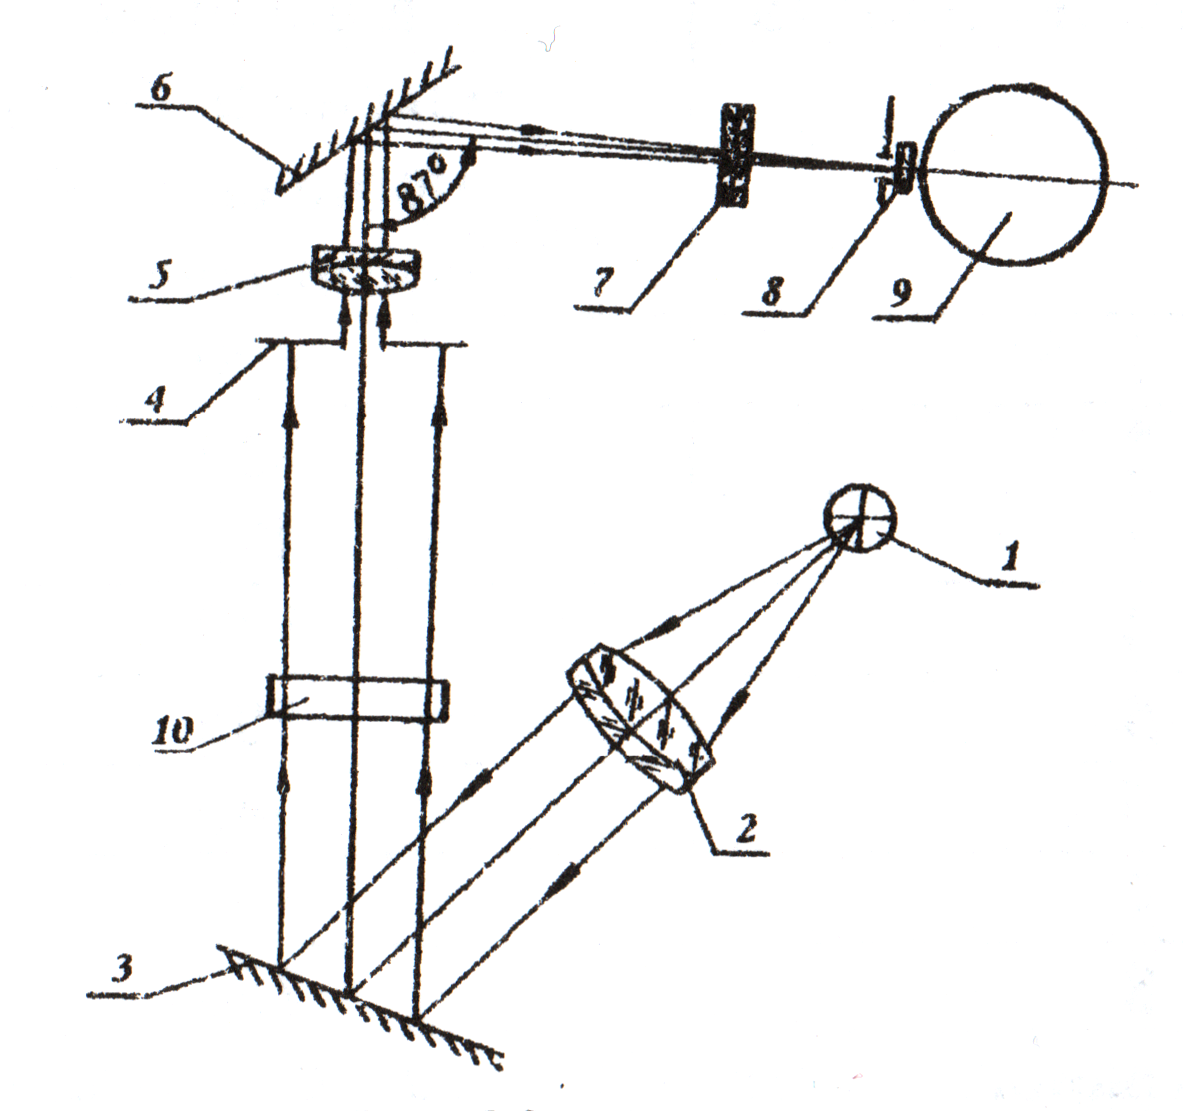
\includegraphics[width=80mm]{img_2}}
\caption{\source{}}
\label{img:2}
\end{figure}

\newpage
\begin{enumerate}
	\item оптичний блок;
	\item регулятор чутливості;
	\item покажчик вимірювальної величини;
	\item мікроамперметр;
	\item головка оптична;
	\item ручка установки електричного нуля;
	\item барабан вимірний;
	\item барабан повороту предметного столика;
	\item блок живлення;
	\item ручка збільшення чутливості;
	\item ручка для встановлення селективного поглинача;
	\item кюветне відділення;
	\item набір світлофільтрів.
\end{enumerate}

\bigskip
\bigskip
\bigskip
\bigskip
\bigskip
\bigskip
\bigskip
\bigskip
\bigskip

\begin{enumerate}
	\item джерело світла;
	\item конденсор;
	\item поворотне дзеркало;
	\item діафрагма;
	\item об'єктив;
	\item поворотне дзеркало;
	\item селективний поглинач;
	\item матове скло;
	\item фотоелемент;
	\item досліджуваний світлофільтр.
\end{enumerate}
\clearpage ~

\begin{figure}[h]
\centering{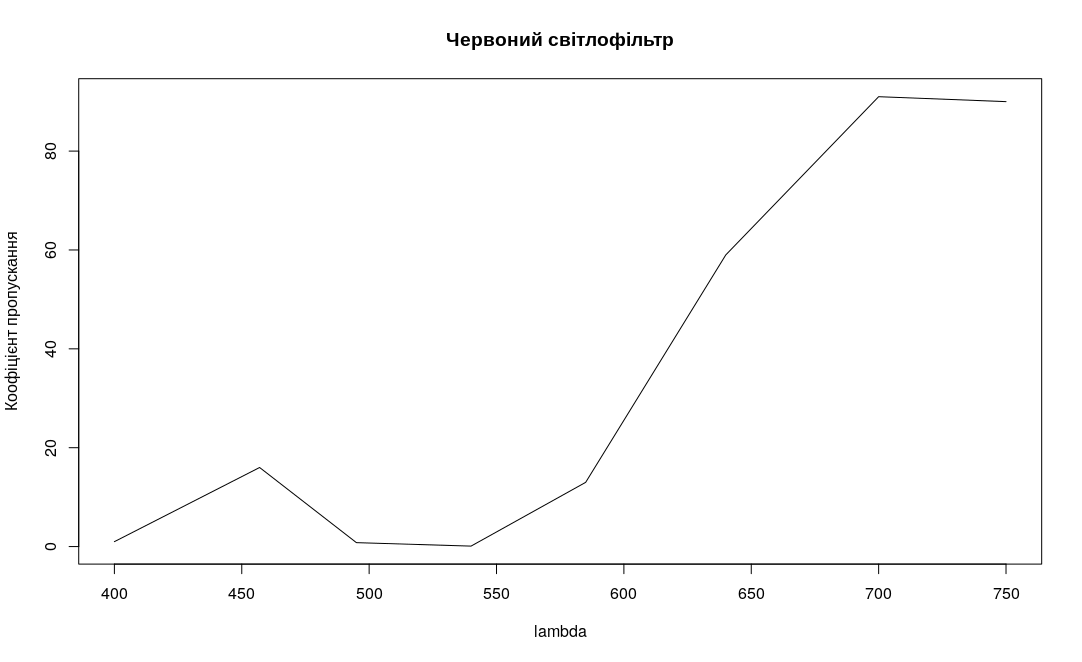
\includegraphics[width=160mm]{red}}
\caption{\source{}}
\label{img:1}
\end{figure}

\begin{figure}[h]
\centering{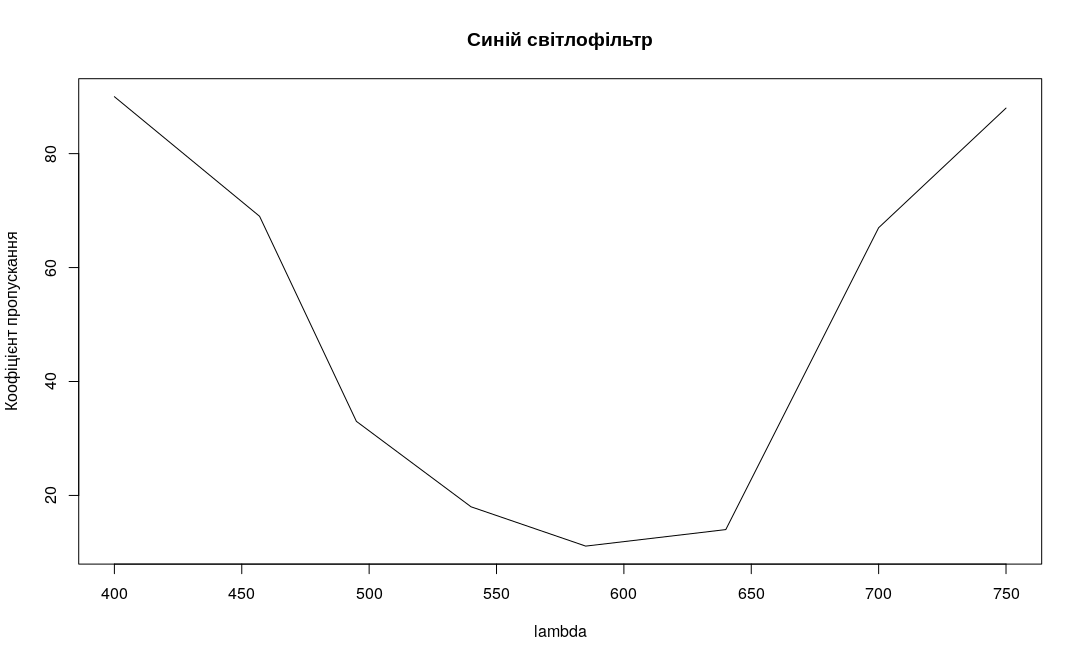
\includegraphics[width=160mm]{blue}}
\caption{\source{}}
\label{img:1}
\end{figure}

\begin{figure}[h]
\centering{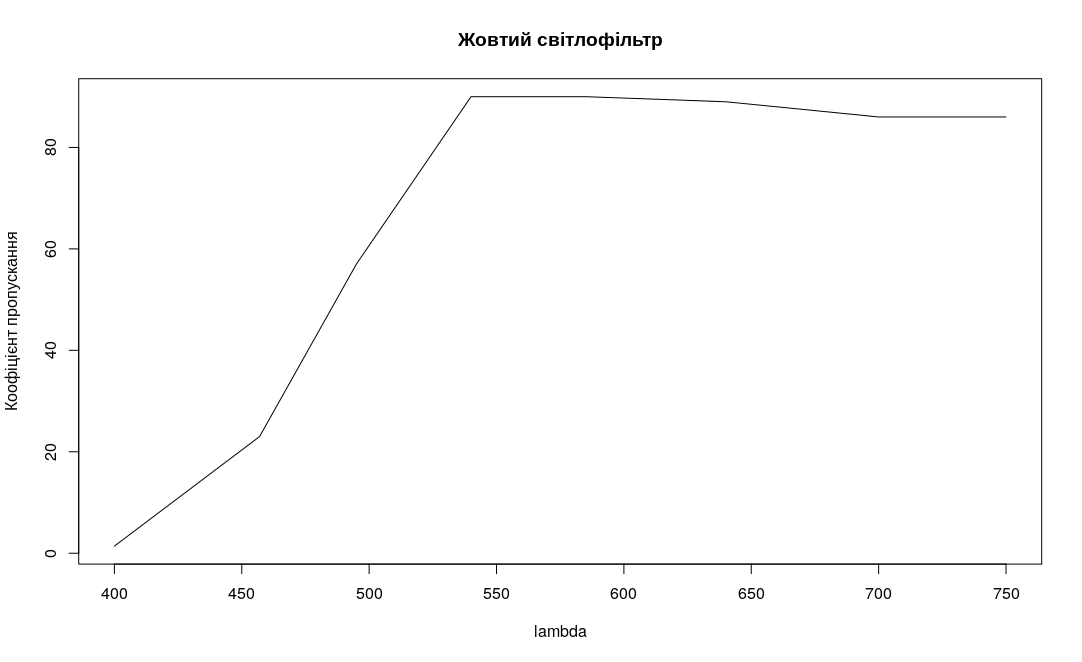
\includegraphics[width=160mm]{yellow}}
\caption{\source{}}
\label{img:1}
\end{figure}

\end{document}



%\begin{table}[b]
%\processtable{Coefficients and remainders for distribution KK ($k = 0.05$,
%$v = 3$, $c_{1} = 1.5$, $c_{2} = 4.5$)}
%{\begin{tabular}{|l|l|l|}\hline
%$n$ & $a_{n}^{2}$ & $r_{k}(1)$\\\hline
%0 & 3.602576748428 & 1.493719547999\\\hline
%1 & 1.384791111989 & 0.108928436101\\\hline
%2 & 0.108600438794 & 0.000327997399\\\hline
%3 & 0.000275794597 & 0.000052202814\\\hline
%4 & 0.000027616892 & 0.000024585922\\\hline
%5 & 0.000018178621 & 0.000006407300\\\hline
%\end{tabular}}{}
%\end{table}
%
%So, the basic preamble and main body will be:
%\verb"\documentclass[twocolumn]{el-author}"\\
%\verb"\usepackage[...]{packages}"\\
%\verb"\date{12 December 2012}"\\
%\verb"\title{...}"\\
%\verb"\author{...}"\\
%\verb"\abstract{...}"\\
%\verb"\maketitle{...}"\\
%\verb"\begin{document}"\\
%\verb"..."\\
%\verb"\section{...}"\\
%\verb"..."\\
%\verb"\section{..}"\\
%\verb"..."\\
%\verb"\end{document}"